\documentclass[
 reprint,
 amsmath,amssymb,
 aps,
]{revtex4-1}

\usepackage{graphicx}  
\usepackage{epstopdf}
\usepackage{dcolumn}
\usepackage{bm}	
\usepackage{amsmath}			
\usepackage{amsfonts}			
\usepackage{amssymb}			
\usepackage{latexsym}		
\usepackage{color}

\begin{document}

\title{Impact of Forward stimulated Brillouin scattering on the propagation of a nanosecond-class and energetic laser pulse}
\author{C. Ruyer}\email{charles.ruyer@cea.fr}
\author{A. Debayle}
\author{P. Loiseau}
\author{M. Casanova}
\author{P. E. Masson-Laborde}
\affiliation{CEA, DAM, DIF, F-91297 Arpajon, France}

\begin{abstract}
\end{abstract}

\maketitle

\section{Introduction}

\section{The theory}
\subsection{Pump wave and diffusion of  laser fields}
Following the developments of Refs. \cite[]{phd-Grech,PRL_Grech_2009}, we start by an electric field with a main propagation direction lying on the $x$-axis, a broad transverse spatial spectrum and two frequencies, $\omega_p$ and $\omega_d$ for the pump and diffused wave  respectively.  Note that the vectors are noted in bold symbols. Introducing, $D=1$ or $2$, the number of transverse direction, we assume that the electric field in real space that depends on space and time, $\mathbf{r}$  and $t$ respectively, reads
\begin{align}
E(\mathbf{r},t)= \Re \Big[ \int \frac{d^Dk_p}{(2\pi)^D} E_p (\mathbf{k}_p,t) e^{i \mathbf{k}_p \cdot \mathbf{r}_\perp} \nonumber \\
+\int \frac{d^Dk_d}{(2\pi)^D} E_d (\mathbf{k}_d,t) e^{i \mathbf{k}_d \cdot \mathbf{r}_\perp -i (\omega_d - \omega_p)t}   \Big] \, ,
\end{align}
where the subscript $\perp$ designate the transverse direction ($y,z$ and $y$ in three and two dimension respectively)  components and $\Re$  ($\Im$) the real (imaginary) part of a complex. Note that electric field, as written above,  has already been enveloped in time and space around $\omega_p$ and $k_0$ so that the physical one should be multiplied  by $\exp(k_0 x-i\omega_p t)$.

In the transverse Fourier space, dropping the dependence in time and $x$ for simplicity and with $\omega_s=\omega_d - \omega_p$,
\begin{align}
E(\mathbf{k}) =     E_p(\mathbf{k})
+  E_d(\mathbf{k}) e^{ -i \omega_s t}   \, .
\end{align} 
Using $I(k)=c\epsilon_0 \int E(k_p) E(k-k_p) dk_p$, we may split the total intensity in a pump intensity $I_p$ and diffused one $I_d$ verifying to leading order in $E_d$, \emph{i.e.} for $\vert E_d\vert \ll \vert E_p \vert$, 
\begin{align}
I(\mathbf{k}) &=I_p(\mathbf{k})+I_d(\mathbf{k})\, , \label{eq:itot}\\
I_p(\mathbf{k}_p) &=   \frac{c\epsilon_0}{2} \int E_p(\mathbf{k}) E_p^\star(\mathbf{k}_p-\mathbf{k}) d^Dk \, , \label{eq:ip} \\
I_d(\mathbf{k}_d) &\simeq   c\epsilon_0  \Re \int E_p(\mathbf{k}) E_d^\star(\mathbf{k}_d-\mathbf{k})e^{i\omega_s t } d^Dk \, , \label{eq:id}
\end{align}
with $\epsilon_0$ and  $c$, the electric permittivity and speed of light in vacuum.
In this study we will only consider wavevectors cloth to the initial
propagation direction ($x$) and note $\mathbf{k}_{p/d}=k_0\hat{\mathbf{x}} +k_{p/d,\perp}\hat{\mathbf{r}_\perp}  $ where $\hat{\mathbf{x}}$ and $\hat{\mathbf{r}_\perp}$ are unity vectors in the $x$ and transverse directions respectively. Hence, $\omega_p^2 = \omega_{pe}^2+ \mathbf{k}_p^2c^2$ and $\omega_d^2 = \omega_{pe}^2+\mathbf{k}_d^2c^2$ where $\omega_{ps}$ is the $s$-species plasma frequency and the susbscripts $e,i$ corresponds the the electrons and ions respectively.

Hence, for a pump  diffusion that occurs close to the $x$-axis,  \emph{i.e.}  $\vert \mathbf{k}_p -\mathbf{k}_d\vert \ll k_0$ and we may write to leading order the plasma wave frequency frequency and wavevector,
\begin{align}
\omega_s=\omega_p-\omega_d&= -(\mathbf{k}_s^2 c^2-2\mathbf{k}_p\cdot\mathbf{k}_s c^2)/2\omega_0
\, , \nonumber\\
\mathbf{k}_s& = \mathbf{k}_p-\mathbf{k}_d\, ,
\end{align}
where $\omega_0^2= \omega_{pe}^2+ k_0^2c^2$.
Hereafter, we will assume that the plasma wave remain mainly transverse to the pump so that $\mathbf{k}_s=k_s \hat{\mathbf{r}_\perp}$ and $ \vert \mathbf{k}_p\cdot\mathbf{k}_s\vert \ll k_s^2$. 
Hence, use will be made of 
\begin{align}
\omega_s  &= -\frac{k_s^2 c^2 }{2\omega_0} \, ,\label{eq:ws}\\
\frac{\omega_s}{k_s}& = -\frac{k_s c^2 }{2\omega_0} \label{eq:vphis} \, .
\end{align}
Noticing $k_s/k_0\equiv \sin(\theta) $, one recover the vastly used  relation giving, as a function of the incident angle of two plane waves, the phase speed of the  diffraction pattern of interest in the case of cross-beam energy transfer (CBET) \cite[]{POP_Debayle_2018}.

Introducing the laser critical density, $n_c = m_e \epsilon_0c^2 k_0^2/q_e^2 $ (where  $m_e$ and  $q_e$ are the  electron mass and charge respectively), the  paraxial propagation equation of the electric field verifies 
\begin{equation}
    \partial_x E(t) +\frac{i\mathbf{k}^2}{2k_0}E=\frac{-ik_0n_0}{2n_c} \int \frac{d^Dk_s}{(2\pi)^D} \frac{\delta n(t,\mathbf{k}_s)}{n} E(t,\mathbf{k}-\mathbf{k}_s) \, ,\label{eq:parax}
\end{equation}
which includes diffraction through the second term of the left-hand side.  
The right-hand side models the  diffusion  of the pump wave  on the broad spectrum density fluctuations ($\delta n/n$).

At this stage it is crucial to  account correctly for the plasma response to the beating between  the pump and the diffused electromagnetic wave. 

\subsection{Plasma response to a driven wave}
As will be shown subsequently, no monochromatic approximation can be made regarding $E_d(k_d)$ or $\delta n(k_s)/n$, like for the cases of backward Brillouin scattering. Instead, the density fluctuations are the  result of the superposition of many diffraction patterns characterized by there wavevector $k_s$ and with different  phase speeds [see Eq. \eqref{eq:vphis}].

For a given set of $k_p$, $k_s$, $\omega_p$ and $\omega_s$, Eq. (12) of  Ref. \cite[]{POF_Drake_1973} shows that  for  a Maxwellian plasma, the plasma response to a drive  takes on 
\begin{align}
 \frac{ \delta n (\omega_s, k_p,k_s) }{n}  &=   \frac{ -\epsilon_0 E_p(k_p) E_d(k_p-k_s) }{ 4 n_c T_e } \nonumber \\  &\times \alpha_\mathrm{kin}\left(\frac{\omega_s- \mathbf{k}_s\cdot \mathbf{v}_d}{\vert \mathbf{k}_s \vert }\right)   \, ,\label{eq:drake}
 \end{align}
 where, for an electron Debye length $\lambda_{De}$ that verifies $\vert k_s \lambda_{De} \vert \ll 1$, %in the case of only one transverse direction ($D=1$), 
 \begin{align}
\alpha_\mathrm{kin} &=  \frac{-1}{2}\frac{ \mathcal{Z}'( \xi_e)\mathcal{Z}'( \xi_i)    }{   \mathcal{Z}'( \xi_i) - \mathcal{Z}'( \xi_e)\frac{  T_i }{ ZT_e } }    \, , \label{eq:drakea}\\
\xi_{e/i } &=  \sqrt{ \frac{ m_{e/i } }{ 2T_{e/i }}  } \left( \frac{ -\vert \mathbf{k}_s\vert c^2  }{  2\omega_0 }  - \frac{    \mathbf{k}_s \cdot \mathbf{v}_d }{  \vert \mathbf{k}_s\vert }\right)  \label{eq:xiie}   \,  .
%\xi_{e/i } &=  \sqrt{ \frac{ m_{e/i } }{ 2T_{e/i }}  } \left( \frac{ -\vert \mathbf{k}_s\vert c^2  }{  2\omega_0 }+\frac{  2\mathbf{k}_{p,\perp}\cdot \mathbf{k}_sc^2 }{  2\vert k_s \vert \omega_0 }  - \frac{    \mathbf{k}_s \cdot \mathbf{v}_d }{  \vert \mathbf{k}_s\vert }\right)  \label{eq:xiie}   \,  .
\end{align}
We introduced $Z$, the ion charge number and  $ \mathcal{Z}$, the plasma dispersion function \cite{Fried_Gell-Mann_1960} and its arguments $\xi_{e } $ and $\xi_{i }$, which in turns depend on $T_{e,i}$ and $v_d$, the electron/ion temperature and  drift velocity.

In order to be combined with the paraxial description of light propagation of Eq. \eqref{eq:parax}, one needs to apply in temporal inverse Fourier transform of Eq. \eqref{eq:drake}. We will account for both stokes $\omega=\omega_s$ and anti-stokes modes $\omega=-\omega_s$ giving 
\begin{equation}\label{eq:sa}
     \frac{ \delta n (t) }{n}= \frac{ \delta n (\omega_s) }{n}e^{-i\omega_st} + \frac{ \delta n (-\omega_s) }{n}e^{i\omega_st}\, .
\end{equation}

We may now use $\alpha_\mathrm{kin}(-x) = \alpha^\star_\mathrm{kin}(x) $ to recast the above formula as 
\begin{align}
\frac{ \delta n (t,k_p,k_s ) }{n}  &=   \frac{ -\epsilon_0 E_p(k_p) E_d(k_p-k_s)  }{ 2 v_g n_c T_e } 
 \Re \left[ \alpha_\mathrm{kin}  e^{ i\omega_s(k_s) t} \right]  \, .\label{eq:drakef}
\end{align}

Note that the term inside the real part only depends on $k_s$:   a summation of the above relation over $k_p$ results, using Eq. \eqref{eq:id}, in  
\begin{align}
\frac{ \delta n (t,k_s ) }{n}  &=   \frac{ -I_d(k_s) }{ 2 v_g n_c T_e } 
 \Re \left( \alpha_\mathrm{kin}   \right)  \, .\label{eq:drakef}
\end{align}

\begin{figure}
\begin{tabular}{c}
(a) $D=1$\\
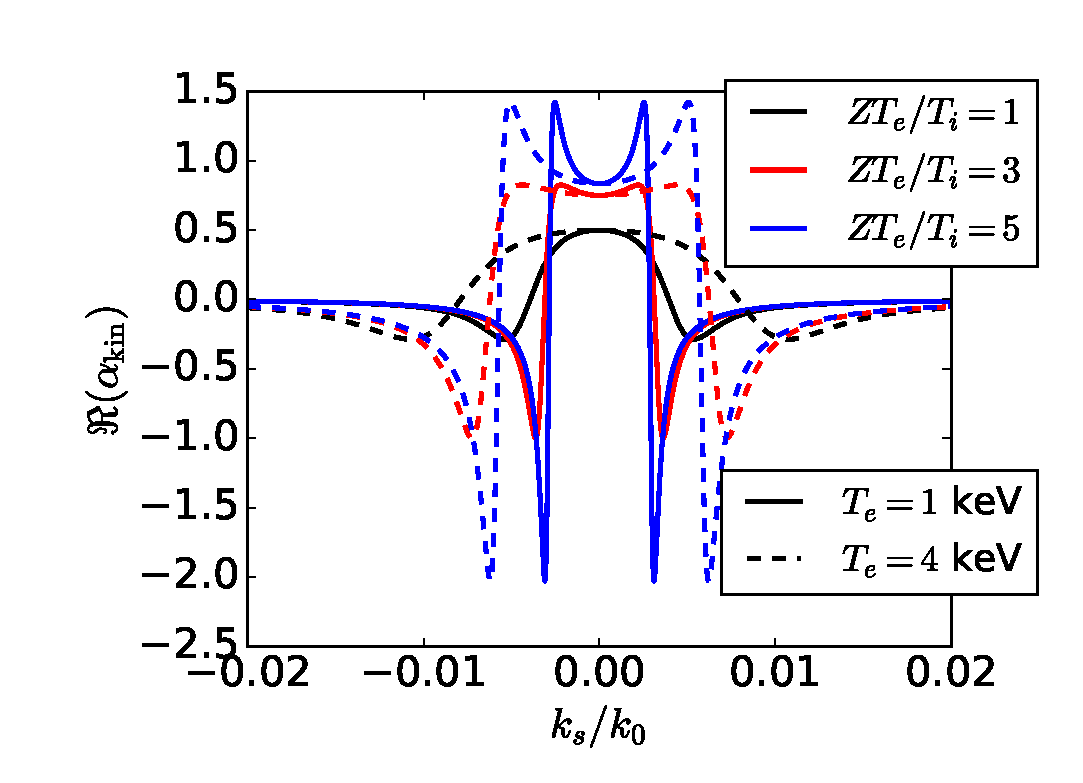
\includegraphics[width=0.49\textwidth]{akin.eps}\\
(b) $D=2$\\
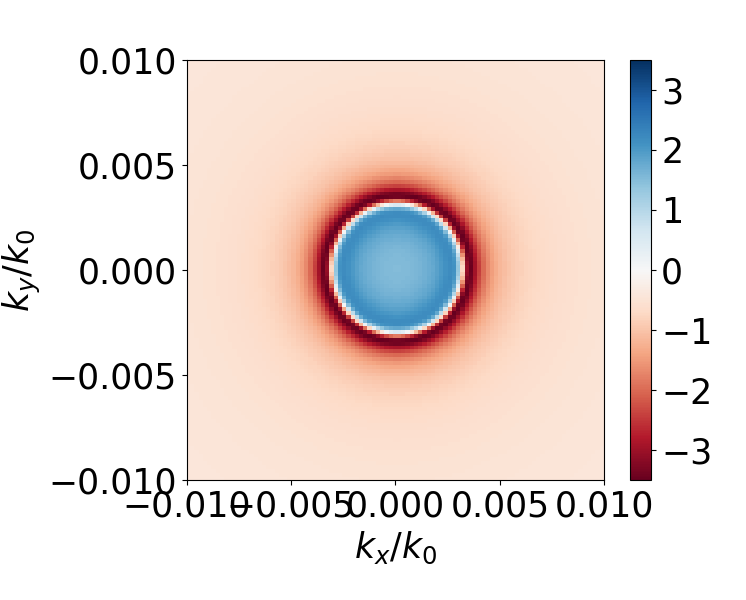
\includegraphics[width=0.49\textwidth]{real_F_kin_3d_vd0cs_te1keV_Ti300eV_H+.png}\\
(c) $\alpha_r^{(n)}$ for  $D=1$\\
\end{tabular}
\caption{ \label{fig:akin}  
 $\Re \left( \alpha_\mathrm{kin}   \right)$ for $D=1$ (a) and $D=2$ (b) as function of $k_s/k_0$ for a H$^{+}$ plasma with $n_0=0.1n_c$, $T_e =1$ keV for various $ZT_e/T_i$. 
 }
\end{figure}
In a 2D system ($D=1$), Fig. \ref{fig:akin} illustrates, for $D=1$ and for  a H$^{+}$ plasma with $n_0=0.1n_c$ and  $T_e =1$ keV, that $\Re \left( \alpha_\mathrm{kin}   \right)$ is an even function  of $k_s/k_0$ of width that enlarges as  $ZT_e/T_i$ increases. Moreover, its value vanishes for $\vert k_s/k_0 \vert  \gtrsim 2 \cdot 10^{-2}$, showing that the plasma is sensitive  to the very large wavelength perturbations ($\lambda_s/\lambda_0=k_0/k_s\gtrsim 314 $ or $k_s/k_0\lesssim 0.02$). As there is, in  the system of interest here no privileged scattering direction, both stokes and antistokes plasma response modes have to be taken into account [see Eq. \eqref{eq:sa}]. Hence,  the resulting diffraction pattern  in the case of FSBS is  a stationary  wave, unlike CBET where it is fully propagating.


\subsection{Derivation of an effective growth rate relevant for an  RPP beam}
 \begin{widetext}
We may now combine the kinetic plasma response  with the paraxial model of  the laser propagation. 
However, it  is easier at this stage to introduce $\Bar{E}$ with  $E=\Bar{E}\exp(-i \mathbf{k}^2x /2k_0)$ so that Eq. \eqref{eq:parax} becomes
\begin{equation}
    \partial_x \Bar{E}  =\frac{-ik_0n_0}{2n_c} e^{\frac{i\mathbf{k}^2x }{2k_0}}\int \frac{d^Dk_s}{(2\pi)^D} \frac{\delta n(\mathbf{k}_s)}{n} \Bar{E}(\mathbf{k}-\mathbf{k}_s) e^{ \frac{-i(\mathbf{k}-\mathbf{k}_s)^2x}{2k_0}}\, ,  \label{eq:paraxbar}
\end{equation}
 plugged in Eq. \eqref{eq:drakef}, we obtain
\begin{align}
    \partial_x \Bar{E}  =\frac{ik_0n_0}{4n_c} \frac{e^{\frac{i\mathbf{k}^2 x}{2k_0}}}{  v_g n_c T_e}
    %\times \nonumber \\
    \int \frac{d^Dk_s}{(2\pi)^D}  e^{ \frac{-i(\mathbf{k}-\mathbf{k}_s)^2x}{2k_0}} \Bar{E}(\mathbf{k}-\mathbf{k}_s) 
   I_d(\mathbf{k}_s) \alpha_\mathrm{r}   (\mathbf{k}_s) \, ,  \label{eq:paraxbar}
\end{align}
where we introduced $\alpha_\mathrm{r}=\Re(\alpha_\mathrm{kin} )$ and $\beta_r$. 

%\onecolumngrid
 When retaining only the first order terms (as $E_d$ and $I_d$, $I_p$ and $E_p$ are considered of order zero), we obtain 
 \begin{align}
   e^{-i\omega_s t}\partial_x \Bar{E}_d  =\frac{ik_0n_0}{4n_c} \frac{e^{\frac{i\mathbf{k}^2 x}{2k_0}}}{  v_g n_c T_e} \times 
   \int \frac{d^Dk_s}{(2\pi)^D} 
   e^{ \frac{-i(\mathbf{k}-\mathbf{k}_s)^2x}{2k_0}}
   I_d(\mathbf{k}_s) \alpha_\mathrm{r}   (\mathbf{k}_s) \Bar{E}_p(\mathbf{k}-\mathbf{k}_s) 
   \, .  \label{eq:paraxbar}
\end{align}

In order to shade light on the dependence of the diffusion growth on the laser energy scattering direction, one needs to combine the above relation with the definition of $I_d(\mathbf{k})$ of  Eqs. \eqref{eq:ip}-\eqref{eq:id}, which can be recast as,
\begin{align}
I_d(\mathbf{k}_d) &\simeq  \Re\left[  c\epsilon_0e^{\frac{ i\mathbf{k}_d^2x}{2k_0}}  \int d^Dk \Bar{E}_d(\mathbf{k}) \Bar{E}_p^\star(\mathbf{k}_d-\mathbf{k})e^{-i\omega_s t -\frac{i2\mathbf{k}_d\cdot \mathbf{k}x}{2k_0}}\right]  \, , \label{eq:idb} \\
I_p(\mathbf{k}_d) &\simeq  \Re\left[  \frac{c\epsilon_0}{2}e^{\frac{ i\mathbf{k}_d^2x}{2k_0}}  \int d^Dk \Bar{E}_p(\mathbf{k}) \Bar{E}_p^\star(\mathbf{k}_d-\mathbf{k})e^{ -\frac{i2\mathbf{k}_d\cdot \mathbf{k}x}{2k_0}}\right]  \, , \label{eq:ipb}
\end{align}
hence
\begin{align}
\partial_xI_d(\mathbf{k}_d)=  &  c\epsilon_0  \Re\left( \int d^Dk e^{-i\omega_st+ \frac{i( \mathbf{k}_d^2-2\mathbf{k}_d\cdot \mathbf{k} )x}{2k_0}} \Bar{E}_p^\star(\mathbf{k}_d-\mathbf{k} )
\left[\partial_x \Bar{E}_d (\mathbf{k}  ) 
+i\frac{  \mathbf{k}_d^2-2\mathbf{k}_d\cdot \mathbf{k}}{2k_0} \Bar{E}_d(\mathbf{k})
\right]  \right)\, , \label{eq:idbdz}
\end{align}
where the variations along $x$ of $\Bar{E}_p$ were neglected. 
The  use of Eq. \eqref{eq:paraxbar} yields, 
\begin{align}
\partial_xI_d(\mathbf{k}_d)\simeq &\Re\Big( \frac{ik_0n_0}{4n_c} \frac{c\epsilon_0 }{  v_g n_c T_e}   \int d^Dk \int \frac{d^Dk_s}{(2\pi)^D} \Bar{E}_p^\star(\mathbf{k}_d-\mathbf{k})
e^{\frac{-i(\mathbf{k}-\mathbf{k}_s)^2x}{2k_0} }
e^{\frac{i(\mathbf{k}_d-\mathbf{k})^2x}{2k_0} }
I_d(\mathbf{k}_s) \alpha_\mathrm{r}(\mathbf{k}_s) 
\Bar{E}_p(\mathbf{k}-\mathbf{k}_s) 
 \Big) \nonumber\\
& +c\epsilon_0  \Re\left( \int d^Dk e^{-i\omega_s t+\frac{ i( \mathbf{k}_d^2-2\mathbf{k}_d\cdot \mathbf{k} )x}{2k_0}} 
i\frac{  \mathbf{k}_d^2-2\mathbf{k}_d\cdot \mathbf{k}}{2k_0} \Bar{E}_d(\mathbf{k})\Bar{E}_p^\star(\mathbf{k}_d-\mathbf{k} )
  \right)
\, . \label{eq:g1}
\end{align}
We may now use Eqs. \eqref{eq:idb} and  \eqref{eq:ipb}, 
\begin{align}
\partial_xI_d(\mathbf{k}_d)\simeq \Re\Big( \frac{ik_0n_0}{4n_c} \frac{1 }{  v_g n_c T_e}    \int \frac{d^Dk_s}{(2\pi)^D} I_d(\mathbf{k}_s) \alpha_\mathrm{r}(\mathbf{k}_s)
I_p(\mathbf{k}_d-\mathbf{k}_s)
+\frac{i\mathbf{k}_d^2}{2k_0} I_d \Big) 
  \nonumber\\
 +c\epsilon_0  \Re\left( \int d^Dk e^{-i\omega_s t+\frac{ i( \mathbf{k}_d^2-2\mathbf{k}_d\cdot \mathbf{k} )x}{2k_0}} 
i\frac{ -2\mathbf{k}_d\cdot \mathbf{k}}{2k_0} \Bar{E}_d(\mathbf{k})\Bar{E}_p^\star(\mathbf{k}_d-\mathbf{k} )
  \right)
\, . \label{eq:g2}
\end{align}
For symmetric scattering, the last term  of the above equation may be neglected and, defining $\Bar{I}_d$ through $I_d = \Re[\Bar{I}_d\exp(i\mathbf{k}_d^2x/2k_0)]$, one obtains
 \begin{align}
\partial_x\Bar{I}_d(\mathbf{k}_d)\simeq  \frac{ik_0n_0}{2n_c} \frac{e^{\frac{-i\mathbf{k}_d^2x}{2k_0}} }{  v_g n_c T_e}   
  \int \frac{d^Dk_s}{(2\pi)^D} \Bar{I}_d(\mathbf{k}_s) \alpha_\mathrm{r}(\mathbf{k}_s) 
I_p(\mathbf{k}_d-\mathbf{k}_s)
e^{\frac{i\mathbf{k}_s^2x}{2k_0}} 
\, . \label{eq:g3}
\end{align}
 
 \subsection{Energy growth of the Forward Brillouin scattering for an RPP beam }
 For a RPP pump beam that follows around the focal spot, 
   \begin{align}
   I_p(\mathbf{k}) &= I_0 \sigma ^D \mathcal{H}^{(D)}(\mathbf{k})  &\,  \mathrm{with} \, ,\\ 
   \mathcal{H}^{(1)}(\mathbf{k}) &= H(2k_m - \vert k_y \vert ) &\,  \mathrm{in}\, \mathrm{2D} \, ,\\ 
    \mathcal{H}^{(2)}(\mathbf{k}) &=   H(2k_m - \vert k_y \vert ) H(2k_m - \vert k_z \vert ) &\,  \mathrm{in}\, \mathrm{3D} \, ,
   \end{align} 
     where $H$ is the step function, $k_m=k_0/2f$ with $f$ the effective speckle focal number,  and $\sigma$ the transverse size of the pump wave, \emph{i.e.}, $I_0\sigma^D$ is its initial power.
  \begin{align}
\partial_x\Bar{I}_d(\mathbf{k}_d)\simeq  \frac{ik_0n_0}{2n_c} \frac{e^{\frac{-i\mathbf{k}_d^2x}{2k_0}} }{  v_g n_c T_e}   
 I_0\sigma^D \int \frac{d^Dk_s}{(2\pi)^D}   \mathcal{H}^{(D)}(\mathbf{k}_s) \Bar{I}_d(\mathbf{k}_s) \alpha_\mathrm{r}(\mathbf{k}_s) 
e^{\frac{i\mathbf{k}_s^2x}{2k_0}} 
\, . \label{eq:g4}
\end{align}
Since $2k_m$ is much larger than the width of $\alpha_r(k_s)$, we may use $\int_{k_d-2k_m}^{k_d+2k_m} X \simeq \mathcal{H}^{(D)}(\mathbf{k}) \int_{-\infty}^{+\infty}X$
which, introducing $\delta n/n_c=n_0I_0/{n_c^2 T_ev_g}$, gives
 \begin{align}
\partial_x\Bar{I}_d(\mathbf{k}_d)\simeq  \frac{ik_0}{2}  \frac{\delta n}{n_c}
 \mathcal{H}^{(D)}(\mathbf{k}_d)\sigma^D  \int \frac{d^Dk_s}{(2\pi)^D} \Bar{I}_d(\mathbf{k}_s) \alpha_\mathrm{r}(\mathbf{k}_s) 
e^{\frac{i(\mathbf{k}_s^2-\mathbf{k}_d^2)x}{2k_0}} 
\, . \label{eq:g5}
\end{align}

In order to reach analytical progress, we will assume that $I_d$ is  smoother and larger  than $\alpha_\mathrm{r}(\mathbf{k}_s) 
\exp[i(\mathbf{k}_s^2-\mathbf{k}_d^2)x / 2k_0]$, hence 
\begin{align}
\partial_x\Bar{I}_d(\mathbf{k}_d)\simeq  \frac{ik_0}{2}  \frac{\delta n}{n_c}
 \mathcal{H}^{(D)}(\mathbf{k}_d) \sigma^D \Bar{I}_d(0) \int \frac{d^Dk_s}{(2\pi)^D}  \alpha_\mathrm{r}(\mathbf{k}_s) 
e^{\frac{i(\mathbf{k}_s^2-\mathbf{k}_d^2)x}{2k_0}} 
\, . \label{eq:g6}
\end{align}
 
  \begin{figure*}
\begin{tabular}{cc}
(a) $D=1$ &(b) $D=2$ \\
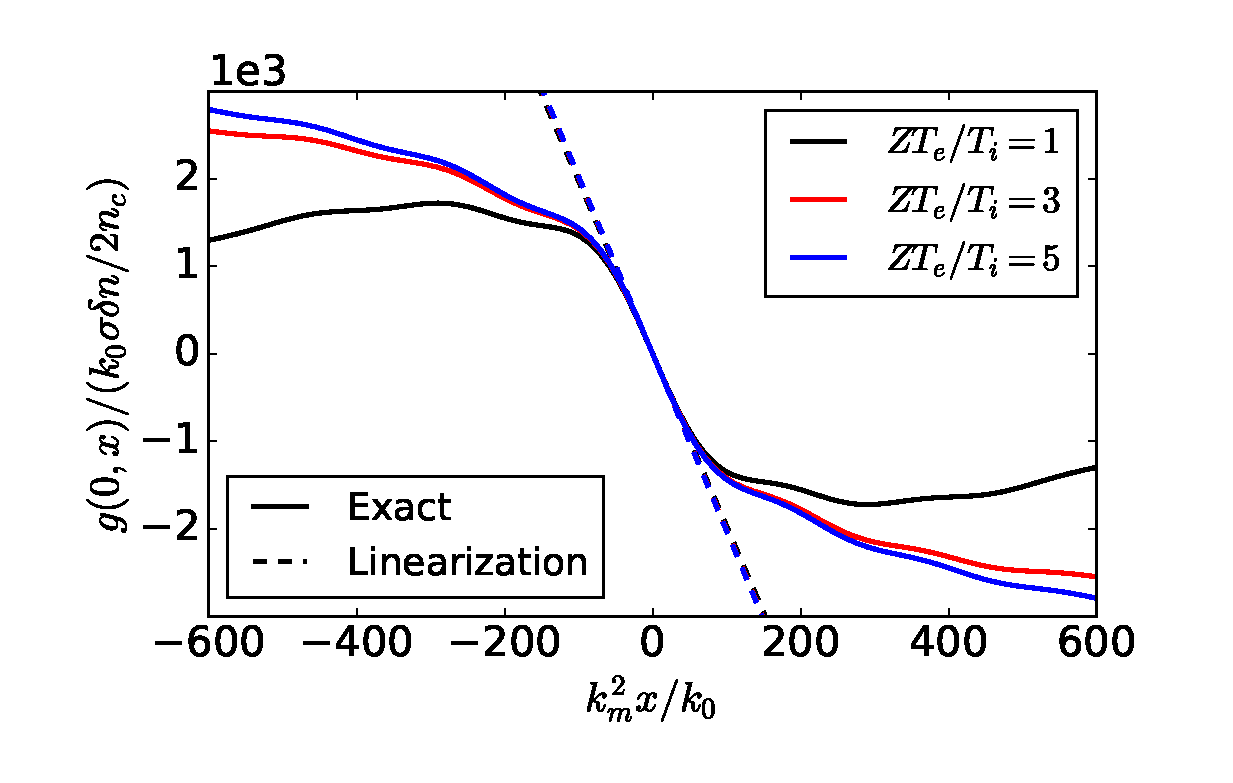
\includegraphics[width=0.49\textwidth]{int_akin_sin.eps}
 &
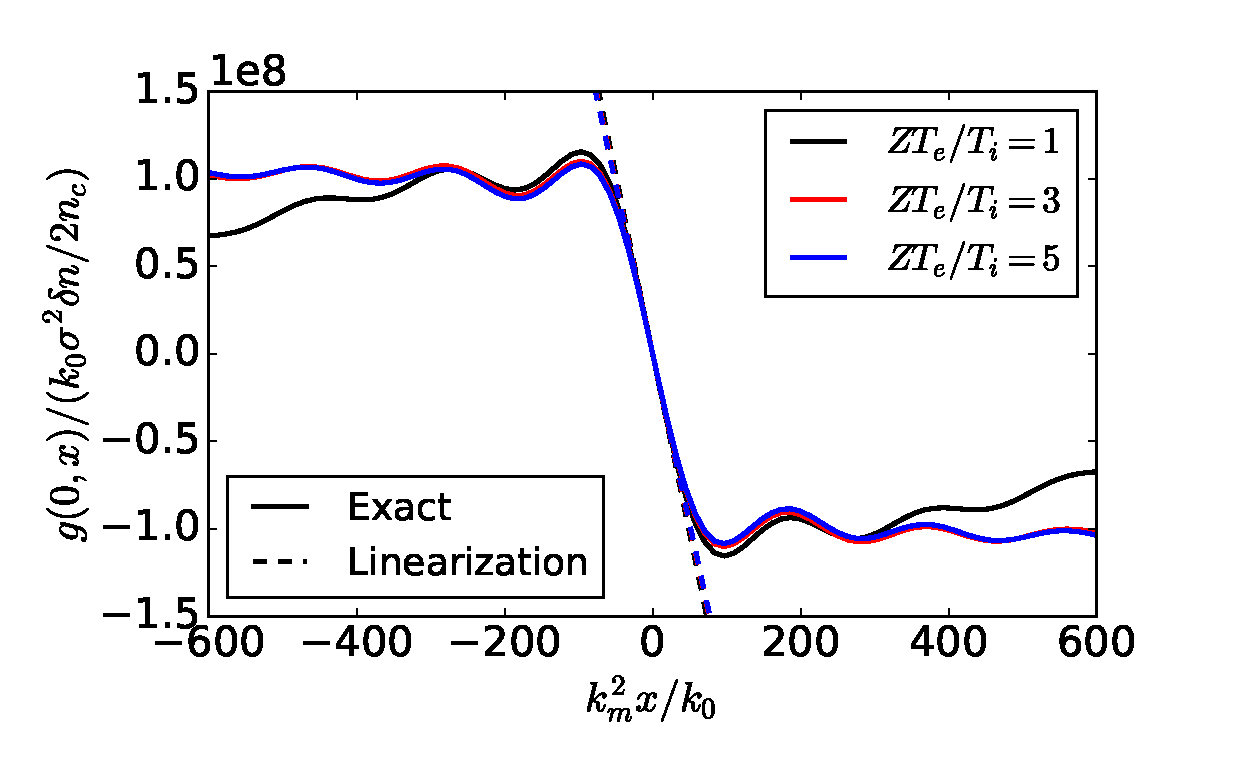
\includegraphics[width=0.49\textwidth]{int_akin_sin_D2.eps}
\end{tabular}
\caption{ \label{fig:intakinsin}
Numerical evaluation of the averaged real gain given by Eq. \eqref{eq:gain0} for various values of $ZT_e/T_i$ in the case $D=1$ (a) and $D=2$ (b) as plain lines for $\sigma = 200 \,\mu m$. The linearization around the focal plane, $x=0$, is superimposed in dashed lines. 
 }
\end{figure*}
An exact and general solution of \eqref{eq:g6} is out of the scope of this manuscript, however, we extract from it some general tendencies such as the averaged growth rate of the energy associated with $I_d$, and the dominant direction in which the pump is scattered. The real part of  Eq. \eqref{eq:g6} leads to the real effective  gain defined following
\begin{align}
&g(\mathbf{k}_d,x) = \Re\left[\frac{\partial_x\Bar{I}_d(\mathbf{k}_d)}{\Bar{I}_d(0)}\right] %\nonumber \\
%&
= - \frac{k_0}{2}  \frac{\delta n}{n_c}
 \mathcal{H}^{(D)}(\mathbf{k}_d)  \sigma^D \int \frac{d^Dk_s}{(2\pi)^D}  \alpha_\mathrm{r}(\mathbf{k}_s) 
\sin\left[ \frac{(\mathbf{k}_s^2-\mathbf{k}_d^2)x}{2k_0}\right]
\, . \label{eq:gainkd}
\end{align}
 \end{widetext}

Hence, the averaged gain can be obtained setting $\mathbf{k}_d=0$,
\begin{align}
g(0,x)&=  -\Gamma_0 \int \frac{d^Dk_s}{(2\pi)^D}  \alpha_\mathrm{r}(\mathbf{k}_s) 
\sin\left[ \frac{\mathbf{k}_s^2 x}{2k_0}\right]\, , \nonumber\\
\Gamma_0&=\frac{k_0}{2}  \frac{\delta n}{n_c}
  \sigma^D \, ,
\label{eq:gain0}
\end{align}
Figures \ref{fig:intakinsin}(a,b) illustrate, as a function of $k_m^2 x /k_0$, the evolution of $g(0,x)$
normalized to $\Gamma_0=k_0\delta n / 2n_c$. Note that, for $\lambda_0=2\pi/k_0=0.35\,\rm\mu m$ and $f=6.5$,  $k_m^2 x /k_0=200$ corresponds to $x\simeq 2\,\rm mm$. 
The averaged energy gain of the diffused wave is positive before focus (\emph{i.e.} $x=0$) and negative afterward, with  a linear behavior of the $g(0,x)$ for  $\vert k_m^2 x /k_0 \vert < 100$  that very weakly depends on $ZT_e/T_i$.  Indeed, as shown in Fig \ref{fig:akin}(c), $\alpha_r^{(2)}$ exhibits no dependence  on $ZT_e/T_i$. Both cases $D=1$ and $2$ present a weaker dependence of $g(0,x)$ on $\vert k_m^2 x /k_0 \vert > 100$, it occurs when the $\sin(k^2x/2k_0)$ in the quadrature of Eq. \eqref{eq:gain0} varies faster than the plateau width of $\alpha_r$, $\vert k_s/k_0\vert \lesssim 5\cdot 10^{-3}\equiv \Delta k /2$ in Figs. \ref{fig:akin}(a,b), \emph{i.e.} for $\vert x\vert \gtrsim k_0/\Delta k^2$ which gives $\vert k_m^2x/k_0 \vert  \gtrsim 60  $ in fair  agreement with Figs. \ref{fig:intakinsin}(a,b).
For $\vert k_m^2 x /k_0 \vert \gtrsim 400$, the absolute value of $g(0,x)$ vanishes faster as $ZT_e/T_i$ decreases. 

Let's momentarily consider, for illustration purposes,  the  case of a RPP beam of width $\sigma =200\,\rm\mu m$, $I_0=3\cdot 10^{14} \,\rm W.cm^{-2}$, $2\pi/k_0 = 0.35\,\rm\mu m$ and $f = 6.5$ propagating in a H$^{+}$ plasma with $n_e/n_c=0.1$, , $T_e=1$ kev and $T_i=300$ eV. In these conditions, $\delta n/n_c \simeq 7\cdot 10^{-4}$ and  for $D=1$ [see Fig. \ref{fig:intakinsin}(a)], one have $g(0,x)/\Gamma_0 \gtrsim 3\cdot 10^3$ before focus (for $200< k_m^2 x/k_0 < 600$) so that, for  a propagation of $\Delta x = 2\,\rm mm$ (\emph{i.e.} $k_m^2 \Delta x/k_0 = 200$), the net gain is $g(0,x)\Delta x\gtrsim 3.5 $. When $D=2$ [see Fig. \ref{fig:intakinsin}(b)], one obtains $g(0,x)\Delta x\gtrsim 70 $, thus yielding substantial growth for both $D=1$ and $2$.

We therefore know that the Forward Brillouin may grow significantly in the plasmas  of interest here and, in order to shade light on the scattered  direction of the pump wave, we will now address the spectral behavior of Eq. \eqref{eq:gainkd}.

\subsection{Angular spread through Forward Brillouin scattering}

Introducing $x_0$, the left boundary of our system, we may now the solution of Eq. \eqref{eq:gainkd}, 
\begin{align}
\partial_x\Bar{I}_d &=\Gamma_0 K  \mathcal{H}^{(D)}(\mathbf{k}_d) g(0,x)
e^{\Gamma_0 G(0,x)-\frac{i\mathbf{k}_d^2 }{2k_0}} \, ,\nonumber\\
G(0,x)&=\int_{x_0}^{x}g(0,x) dx \, , \label{eq:dxidkd}
\end{align}
where $K$ is an integration constant. 

The averaged spectral width, $\Delta k$ or opening angle $\Delta k/k_0 $ may be derived from  
 \begin{align}
 \Delta k ^2(x) = \frac{\int  d^Dk \mathbf{k}^2 g(\mathbf{k},x )}{\int  d^Dk  g(\mathbf{k},x )}\, ,
\end{align}
which reads 
 \begin{align}
 \Delta k ^2(x) = \frac{
  \int \frac{d^Dk_s}{(2\pi)^D}  \alpha_\mathrm{r}(\mathbf{k}_s) 
 \int  d^Dk \mathcal{H}^{(D)}(\mathbf{k})\mathbf{k}^2 \sin\left[ \frac{(\mathbf{k}_s^2-\mathbf{k}^2)x}{2k_0}\right]
 }{
  \int \frac{d^Dk_s}{(2\pi)^D}  \alpha_\mathrm{r}(\mathbf{k}_s) 
\int  d^Dk\mathcal{H}^{(D)}(\mathbf{k})\sin\left[ \frac{(\mathbf{k}_s^2-\mathbf{k}^2)x}{2k_0}\right]
 }\, .
\end{align}
Here also, we will make use of the much larger width of $\mathcal{H}^{(D)}(\mathbf{k})$ ($\sim 4k_m = 2k_0/f$) compared to $\alpha_r$ ($\sim 10^{-2}k_0$, see Fig. \ref{fig:akin}).
We may thus apply a Taylor developments in $k_s$ to  the above quadratures thus using, for $D=1$
 \begin{widetext}
\begin{align}
 \int_{-2k_m}^{2k_m}  dk  k^2 \sin\left[ \frac{ (k^2-k_s^2)x}{2k_0}\right] &= -\frac{4k_mk_0}{x}\cos\left(\frac{ 2k_m^2x}{k_0}\right) + \frac{2k_0}{x} \sqrt{\frac{\pi k_0}{x}} \mathrm{C}\left( \sqrt{\frac{x}{\pi k_0}}  2k_m \right)
 + O(k_s^2)\, . \\ 
 \int_{-2k_m}^{2k_m}  dk  \sin\left[ \frac{ (k^2-k_s^2)x}{2k_0}\right] &= 
 \sqrt{\frac{4\pi k_0}{x}} \mathrm{S}\left( \sqrt{\frac{x}{\pi k_0}}  2k_m \right)
  + O(k_s^2)\, . 
\end{align}
and for $D=2$
\begin{align}
 \int_{-2k_m}^{2k_m}  dk_y  \int_{-2k_m}^{2k_m}  dk_z  (k_y^2+k_z^2) \sin\left[ \frac{(k_y^2+k_z^2 -\mathbf{k}_s^2) x}{2k_0}\right]& =  
 \frac{4\pi k_0^2}{x^2} \left[ \sin\left( \frac{ 2k_m^2 x}{k_0} \right) -\frac{ 2k_m^2x}{k_0}\cos\left( \frac{ 2k_m^2x}{k_0}\right) \right]
 + O(\mathbf{k}_s^2)\, , \\
 \int_{-2k_m}^{2k_m}  dk_y  \int_{-2k_m}^{2k_m}  dk_z  \sin\left[ \frac{(k_y^2+k_z^2 -\mathbf{k}_s^2) x}{2k_0}\right] &= 
 \frac{4\pi k_0}{x}\sin^2 \left( \frac{ k_m^2x}{k_0}\right)
  + O(\mathbf{k}_s^2)\, ,
\end{align}
 where $\mathrm{S}$ and $\mathrm{C}$ are the Fresnel S and C integrals. 
 \end{widetext}
 
 Hence, the angular spread of the diffused wave resulting from FSBS,  can be approximated to 
  \begin{align}
 \Delta k ^2(x) = \frac{
 \frac{k_0}{x}  \mathrm{C}\left( \sqrt{\frac{x}{\pi k_0}}  2k_m \right)
 -\frac{2k_m}{\pi}\sqrt{\frac{\pi k_0}{x}}\cos\left(\frac{ 2k_m^2x}{k_0}\right)
 }{
 \mathrm{S}\left( \sqrt{\frac{x}{\pi k_0}}  2k_m \right)
 }\, ,
\end{align}
for $D=1$ and to 
\begin{align}
 \Delta k ^2(x) =  \frac{ k_0}{x} \frac{
 \left[ \sin\left( \frac{ 2k_m^2 x}{k_0} \right) -\frac{ 2k_m^2x}{k_0}\cos\left( \frac{ 2k_m^2x}{k_0}\right) \right]
 }{
\sin^2 \left( \frac{ k_m^2x}{k_0}\right)
 }\, ,
\end{align}
for $D=2$.


\section*{Acknowledgements}
 \textcolor{red}{We acknowledge important discussion with M. Grech.  
 We also acknowledge D. Dureau and the HERA-team for all their work on the HERA code. }
This work has been done under   CEA-DAM and
the simulations were performed using HPC resources at TGCC/CCRT and CEA-DAM/TERA.
\bibliography{biblio}
\end{document}
